\documentclass[11pt]{easymemo}

\SectionNumber
%\BlackAndWhite

\begin{document}

\MakeTitle{2026.10.18}{MultiPieの基底の生成法の改良 (考察中)}{明大理工 楠瀬博明}


\section{前提}
\begin{itemize}
\item 対称操作と一般点のWyckoff位置の順序はITAに合わせており、一対一対応している。
%\item ある群の対称操作とその親の群の対称操作を対応させるとWyckoff位置も対応する。
\end{itemize}

\section{ルートクラスター}

この節ではデカルト座標を用いる。
$O_{\rm h}$および$D_{\rm 6h}$の一般点を含み、なるべく球形に近いクラスターを構成することを考える。
まず、$D_{\rm 6h}$の対称操作を$g_i$ ($i=1,\cdots,24$)とする。
主軸を$z':[111]$、副軸を$x':[\bar{1}10]$, $y':[\bar{1}\bar{1}2]$に変換し
\begin{align}
g_i^{[111]}=R_cg_iR_c^{-1},
\quad
R_c = \begin{pmatrix}
-\frac{1}{\sqrt{2}} & -\frac{1}{\sqrt{6}} & \frac{1}{\sqrt{3}} \\
\frac{1}{\sqrt{2}} & -\frac{1}{\sqrt{6}} & \frac{1}{\sqrt{3}} \\
0 & \frac{2}{\sqrt{6}} & \frac{1}{\sqrt{3}}
\end{pmatrix}
\end{align}
代表点$\bm{x}_0=(x,y,z)$に変換後の対称操作を行って$\bm{x}_i=g_i^{[111]}\bm{x}_0$を定義する。
次に、得られた点群$\bm{x}_i$に$x,y,z$軸周りの$\pi$回転$R_x,R_y,R_z$を行って得られた点群を加える。
これらを$\bm{x}_{i+24}=R_x\bm{x}_i$, $\bm{x}_{i+48}=R_y\bm{x}_i$, $\bm{x}_{i+72}=R_z\bm{x}_i$とする。
以上で、$24\times 4=96$個の点群が得られる。
このクラスターをルートクラスターと呼ぶことにする。
なお、主軸を$[1\bar{1}\bar{1}]$, $[\bar{1}1\bar{1}]$, $[\bar{1}\bar{1}1]$に取った対称操作を$g_i^{[1\bar{1}\bar{1}]}=R_xg_i^{[111]}R_x$, $g_i^{[\bar{1}1\bar{1}]}=R_yg_i^{[111]}R_y$, $g_i^{[\bar{1}\bar{1}1]}=R_zg_i^{[111]}R_z$とすると、$\bm{x}_{i+24}=g_i^{[1\bar{1}\bar{1}]}(R_x\bm{x}_0)$, $\bm{x}_{i+48}=g_i^{[\bar{1}1\bar{1}]}(R_y\bm{x}_0)$, $\bm{x}_{i+72}=g_i^{[\bar{1}\bar{1}1]}(R_z\bm{x}_0)$の関係がある。

ルートクラスターの点群は、$O_{\rm h}$の対称操作$\bar{g}_i$ ($i=1,\cdots,48$)および$[\bar{1}\bar{1}2]$面に関する鏡映$M$を用いて
\begin{align}
\bar{\bm{x}}_i=\bar{g}_i\bm{x}_0,
\quad
\bar{\bm{x}}_{i+48}=\bar{g}_i(M\bm{x}_0),
\quad
M=\begin{pmatrix}
\frac{2}{3} & -\frac{1}{3} & \frac{2}{3} \\ -\frac{1}{3} & \frac{2}{3} & \frac{2}{3} \\ \frac{2}{3} & \frac{2}{3} & -\frac{1}{3}
\end{pmatrix}
\end{align}
のように得られる\footnote{鏡映操作$M$は$\bar{g}_i$を$O_{\rm h}$に含まれない対称操作に変えてしまうので、$\bar{\bm{x}}_{i+48}=M\bar{\bm{x}}_i$は成り立たないことに注意する。}。
$\bm{x}_j$と$\bar{\bm{x}}_j$ ($j=1,\cdots,96$)の並び順は異なるが一対一対応がある。
ルートクラスターを図\ref{fig:vc}に示す。

\begin{figure}[t]
\caption{ルートクラスター。$D_{\rm 6h}$の主軸ごとに色分けした。}
\label{fig:vc}
\begin{center}
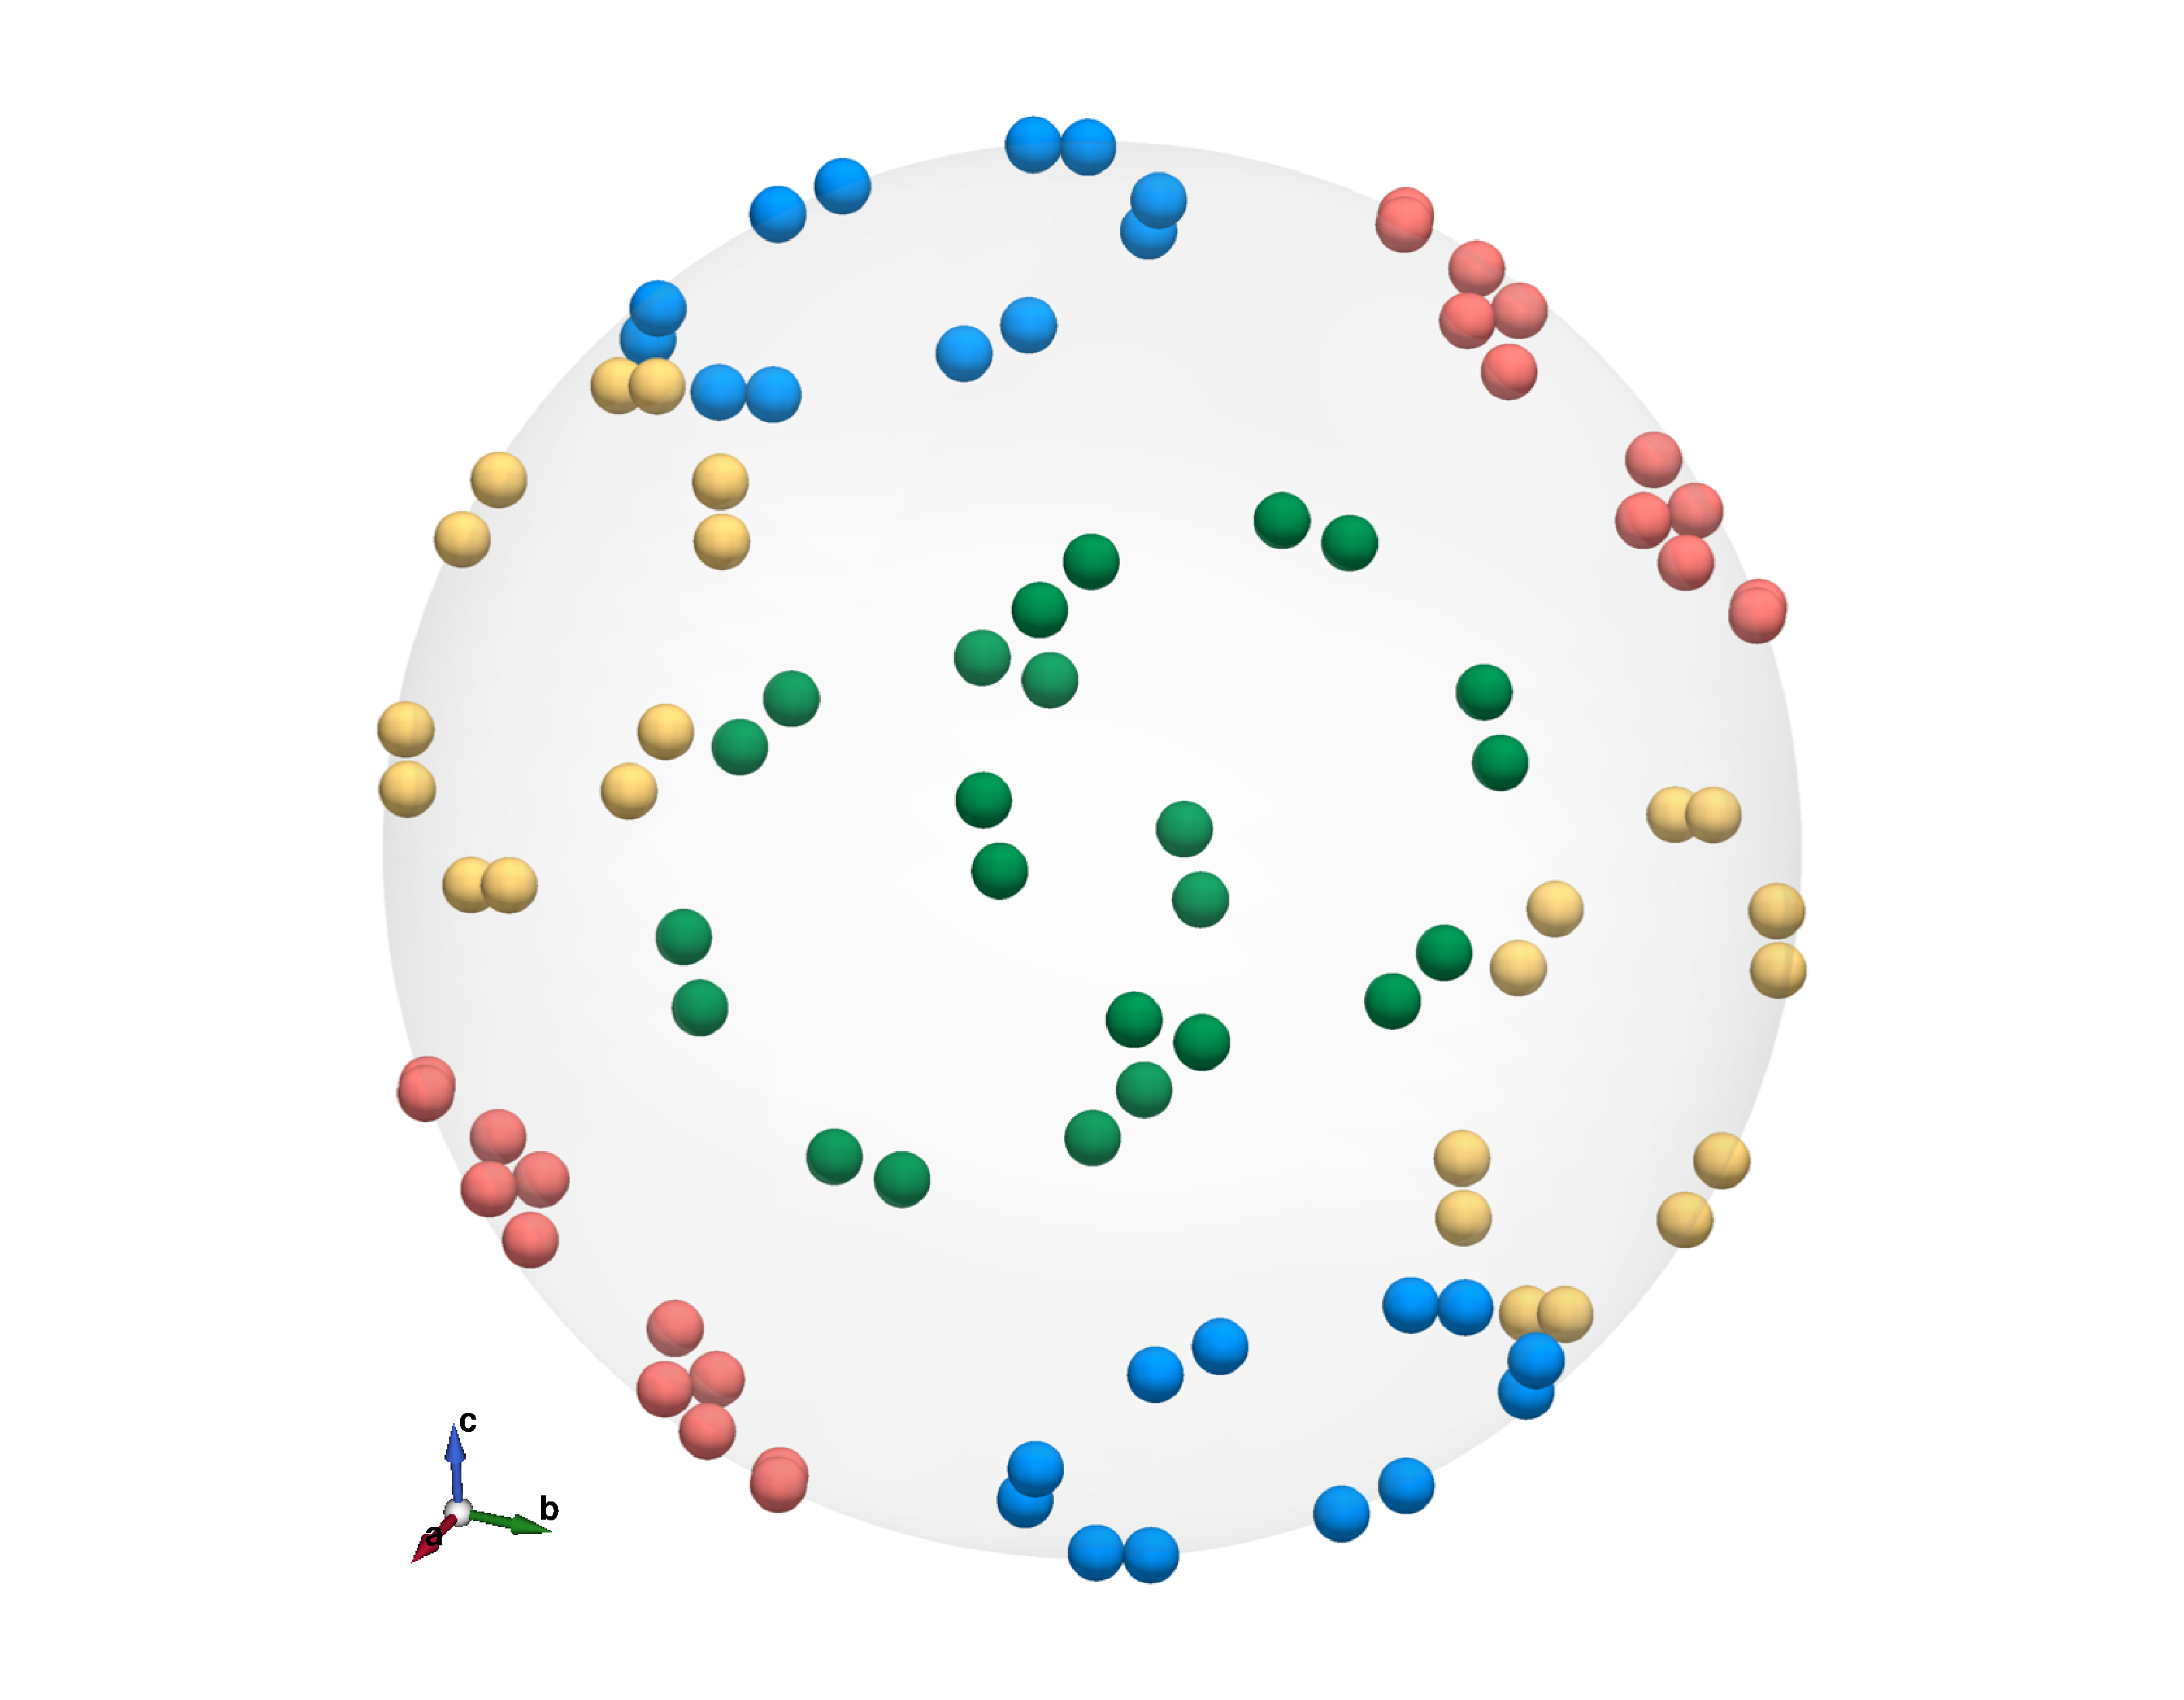
\includegraphics[width=7cm]{vc.eps}
\end{center}
\end{figure}

\section{部分群との関係}

結晶点群は回転群の部分群であり、各結晶点群間にも部分群の関係がある。
親群の対称操作と部分群の対称操作の関係を
\begin{align}
g_{\rm parent}[{\rm coset}[0][i-1]]=\hat{R}\hat{g}_{\rm child}[i-1]\hat{R}^{-1}
\end{align}
と表す。
また、coset[1:]は、部分群に含まれない対称操作を用いて$\hat{g}_{\rm parent}'^{[1:]}({\rm coset}[0])$により得られる。
ここで、$\hat{R}$は主軸変換の行列であり、単位行列になるべく近く、また空間群では原点移動が小さくなるように選ばれている。
親群と部分群の関係を表\ref{tbl:1}に示す。
\begin{align}
&
\hat{R}_c = \begin{pmatrix}
-\frac{1}{\sqrt{2}} & -\frac{1}{\sqrt{6}} & \frac{1}{\sqrt{3}} \\
\frac{1}{\sqrt{2}} & -\frac{1}{\sqrt{6}} & \frac{1}{\sqrt{3}} \\
0 & \frac{2}{\sqrt{6}} & \frac{1}{\sqrt{3}}
\end{pmatrix},
\quad
\hat{R}_{c1} = \begin{pmatrix} -\frac{1}{\sqrt{6}} & \frac{1}{\sqrt{2}} & \frac{1}{\sqrt{3}} \\
-\frac{1}{\sqrt{6}} & -\frac{1}{\sqrt{2}} & \frac{1}{\sqrt{3}} \\
\frac{2}{\sqrt{6}} & 0 & \frac{1}{\sqrt{3}}
\end{pmatrix},
\quad
\hat{R}_t = \begin{pmatrix} \frac{1}{\sqrt{2}} & \frac{1}{\sqrt{2}} & 0 \\
-\frac{1}{\sqrt{2}} & \frac{1}{\sqrt{2}} & 0 \\
0 & 0 & 1
\end{pmatrix}
\cr&
\hat{R}_x = \begin{pmatrix} 1 & 0 & 0 \\ 0 & 0 & 1 \\ 0 & -1 & 0 \end{pmatrix},
\quad
\hat{R}_y = \begin{pmatrix} 0 & 0 & -1 \\ 0 & 1 & 0 \\ 1 & 0 & 0 \end{pmatrix},
\quad
\hat{R}_z = \begin{pmatrix} 0 & 1 & 0 \\ -1 & 0 & 0 \\ 0 & 0 & 1 \end{pmatrix}
\end{align}
また、Cartesin座標系と分率座標系の変換行列は
\begin{align}
T = \begin{pmatrix} 1 & -\frac{1}{2} & 0 \\ 0 & \frac{\sqrt{3}}{2} & 0 \\ 0 & 0 & 1 \end{pmatrix}
\end{align}
である。

すべての結晶点群の一般点はルートクラスターに含まれ、特殊点は一般点を平均化することにより得られる。


\begin{table}[t]
\caption{親群と部分群の関係。}
\label{tbl:1}
\begin{center}
\scriptsize
\begin{tabular}{ccc} \hline\hline
child & parent & c-axis -> p-axis ($\hat{R}$) \\ \hline
C$_1$ & C$_{\rm i}$ & \\
   & C$_2$ & \\
   & C$_{\rm s}$ & \\
   & C$_3$ & \\ \hline
C$_{\rm i}$ & C$_{\rm 2h}$ & \\
   & C$_{\rm 3i}$ & \\ \hline\hline
C$_2$ & C$_{\rm 2h}$ & \\
   & D$_2$ & [010]->[001]:$R_x$ \\
   & C$_{\rm 2v}$ & [010]->[001]:$R_x$ \\
   & C$_4$ & [010]->[001]:$R_x$ \\
   & S$_4$ & [010]->[001]:$R_x$ \\
   & D$_3$ & [010]->[100]:$T^{-1}R_z$ \\
   & D$_3(1)$ & [010]->[120]:$T^{-1}$ \\
   & C$_6$ & [010]->[001]:$T^{-1}R_x$ \\ \hline
C$_{\rm s}$ & C$_{\rm 2h}$ & \\
   & C$_{\rm 2v}$ & \\
   & C$_{\rm 3v}$ & [010]->[100]:$T^{-1}R_z$ \\
   & C$_{\rm 3v}(1)$ & [010]->[120]:$T^{-1}$ \\
   & C$_{\rm 3h}$ & [010]->[001]:$T^{-1}R_x$ \\ \hline
C$_{\rm 2h}$ & D$_{\rm 2h}$ & \\
   & C$_{\rm 4h}$ & [010]->[001]:$R_x$ \\
   & C$_{\rm 6h}$ & [010]->[001]:$T^{-1}R_x$ \\
   & D$_{\rm 3d}$ & [010]->[100]:$T^{-1}R_z$ \\
   & D$_{\rm 3d}(1)$ & [010]->[120]:$T^{-1}$ \\ \hline\hline
D$_2$ & D$_{\rm 2h}$ & \\
   & D$_4$ & \\
   & D$_{\rm 2d}$ & \\
   & D$_{\rm 2d}(1)$ & [100]->[110]:$R_t$ \\
   & D$_6$ & $T^{-1}$ \\
   & T & \\ \hline
C$_{\rm 2v}$ & D$_{\rm 2h}$ & \\
    & C$_{\rm 4v}$ & \\
    & D$_{\rm 2d}$ & [100]->[110]:$R_t$ \\
    & D$_{\rm 2d}(1)$ & \\
    & C$_{\rm 6v}$ & $T^{-1}$ \\
    & D$_{\rm 3h}$ & [010]->[001]:$T^{-1}R_x$ \\
    & D$_{\rm 3h}(1)$ & [100]->[001]:$T^{-1}R_y$ \\ \hline
D$_{\rm 2h}$ & D$_{\rm 4h}$ & \\
    & D$_{\rm 6h}$ & $T^{-1}$ \\
    & T$_{\rm h}$ & \\ \hline\hline
C$_4$ & C$_{\rm 4h}$ & \\
   & D$_4$ & \\
   & C$_{\rm 4v}$ & \\ \hline
S$_4$ & C$_{\rm 4h}$ & \\
   & D$_{\rm 2d}$ & \\
   & D$_{\rm 2d}(1)$ & \\ \hline
C$_{\rm 4h}$ & D$_{\rm 4h}$ & \\ \hline
D$_4$ & D$_{\rm 4h}$ & \\
   & O & \\ \hline
C$_{\rm 4v}$ & D$_{\rm 4h}$ & \\ \hline
D$_{\rm 2d}$ & D$_{\rm 4h}$ & \\
    & T$_{\rm d}$ & \\ \hline,
D$_{\rm 2d}(1)$ & D$_{\rm 4h}$ & \\
      & T$_{\rm d}$ & [100]->[110]:$R_t$ \\ \hline
D$_{\rm 4h}$ & O$_{\rm h}$ & \\ \hline\hline
\end{tabular}
\hspace{1cm}
\begin{tabular}{ccc} \hline\hline
child & parent & c-axis -> p-axis ($\hat{R}$) \\ \hline
C$_3$ & C$_{\rm 3i}$ & \\
   & D$_3$ & \\
   & D$_3(1)$ & \\
   & C$_{\rm 3v}$ & \\
   & C$_{\rm 3v}(1)$ & \\
   & C$_6$ & \\
   & C$_{\rm 3h}$ & \\
   & T & [001]->[111], [100]->[110]:$R_cT$ \\ \hline
C$_{\rm 3i}$ & D$_{\rm 3d}$ & \\
    & D$_{\rm 3d}(1)$ & \\
    & C$_{\rm 6h}$ & \\
    & T$_{\rm h}$ & [001]->[111], [100]->[110]:$R_cT$ \\ \hline
D$_3$ & D$_{\rm 3d}$ & \\
   & D$_{\rm 3d}(1)$ & [100]->[120]:$T^{-1} R_z T$ \\
   & D$_6$ & \\
   & D$_{\rm 3h}$ & [100]->[120]:$T^{-1} R_z T$ \\
   & D$_{\rm 3h}(1)$ & \\
   & O & [001]->[111], [100]->[110]:$R_cT$ \\ \hline
D$_3(1)$ & D$_{\rm 3d}(1)$ & \\
     & D$_{\rm 3d}$ & [100]->[120]:$T^{-1} R_z T$ \\
     & D$_6$ & \\
     & D$_{\rm 3h}$ & \\
     & D$_{\rm 3h}(1)$ & [100]->[120]:$T^{-1} R_z T$ \\
     & O & [001]->[111], [120]->[110]:$R_{c1}T$ \\ \hline
C$_{\rm 3v}$ & D$_{\rm 3d}$ & \\
    & D$_{\rm 3d}(1)$ & [100]->[120]:$T^{-1} R_z T$ \\
    & C$_{\rm 6v}$ & \\
    & D$_{\rm 3h}$ & \\
    & D$_{\rm 3h}(1)$ & [100]->[120]:$T^{-1} R_z T$ \\
    & T$_{\rm d}$ & [001]->[111], [100]->[110]:$R_cT$ \\ \hline
C$_{\rm 3v}(1)$ & D$_{\rm 3d}(1)$ & \\
      & D$_{\rm 3d}$ & [100]->[120]:$T^{-1} R_z T$ \\
      & C$_{\rm 6v}$ & \\
      & D$_{\rm 3h}$ & [100]->[120]:$T^{-1} R_z T$ \\
      & D$_{\rm 3h}(1)$ & \\
      & T$_{\rm d}$ & [001]->[111], [120]->[110]:$R_{c1}T$ \\ \hline
D$_{\rm 3d}$ & D$_{\rm 6h}$ & \\
    & O$_{\rm h}$ & [001]->[111], [100]->[110]:$R_cT$ \\ \hline
D$_{\rm 3d}(1)$ & D$_{\rm 6h}$ & \\
      & O$_{\rm h}$ & [001]->[111], [120]->[110]:$R_{c1}T$ \\ \hline\hline
C$_6$ & C$_{\rm 6h}$ & \\
   & D$_6$ & \\
   & C$_{\rm 6v}$ & \\ \hline
C$_{\rm 3h}$ & C$_{\rm 6h}$ & \\
    & D$_{\rm 3h}$ & \\
    & D$_{\rm 3h}(1)$ & \\ \hline
C$_{\rm 6h}$ & D$_{\rm 6h}$ & \\ \hline
D$_6$ & D$_{\rm 6h}$ & \\ \hline
C$_{\rm 6v}$ & D$_{\rm 6h}$ & \\ \hline
D$_{\rm 3h}$ & D$_{\rm 6h}$ & \\ \hline
D$_{\rm 3h}(1)$ & D$_{\rm 6h}$ & \\ \hline\hline
T & T$_{\rm h}$ & \\
  & O & \\
  & T$_{\rm d}$ & \\ \hline
T$_{\rm h}$ & O$_{\rm h}$ & \\ \hline
O & O$_{\rm h}$ & \\ \hline
T$_{\rm d}$ & O$_{\rm h}$ & \\ \hline\hline
\end{tabular}
\end{center}
\end{table}

Cartesian座標系で点$(x,y,z)$を考える。
O$_{\rm h}$の一般点48点に加えて、これと重ならないD$_{\rm 6h}$の一般点を加える。


--- 以下、考察中メモ ---

この変換を通じて、Wyckoff位置の対応関係を求める。
残りの点群についても一般点の対応関係を求めることができる。
このようにして、32点群のWyckoff位置の対応関係表を作ることができる。
特殊点は一般点の一部なので、対称操作をみれば対応関係を作ることができる。
ボンドも同様。サイトシンメトリーやbond-wyckoffの対応関係、サイトシンメトリーも同様にして得られるはず。
この表ができれば、カイラルペアは対応関係が全く一致する順序で並べておくのがよい。
また、ボンドのSAMBは高対称の群から基底を抜き出して生成し、親のXを引き継ぐ。
このようにすればQ/Gは自動的に定まる。
この生成法はatomicで状態空間を制限するやり方に対応する。

手順をまとめると
\begin{enumerate}
\item 点群の間の一般点Wyckoff位置対応表を作成(site/bond)
\item 特殊点は対称操作マッピングを利用すれば対応が分かる。
\item 対応表にしたがって、高対称のSAMBを縮約していく。Xは引き継ぎ、既約表現は適合関係で決定
\item 直交化
\end{enumerate}
以上により、site/bond-clusterのSAMB一覧ができる。

\[
\hat{Z}_{lm}^{(s,k)}(l_1,l_2)(\hat{\bm{R}})
\equiv\sum_{m_1m_2}C_{l_1m_1,l_2m_2}^{lm}\hat{X}_{lm}^{(s)}(k)O_{l_2m_2}(\bm{R})
\]
これを離散化したものが仮想クラスター上のSAMBである。


\end{document}
